\documentclass{beamer}

% === DATOS === (((
\title{Origami, Teselaciones y Teoría de Conjuntos.}
\author{Erick Rodríguez}
\institute{Universidad Autónoma de Aguascalientes.}
% \date{}
% )))

% === PAQUETES === (((
% \usepackage{wasysym}
\usetheme{Warsaw}
\setbeamertemplate{enumerate items}[circle] % esto lo estoy usando para los simbolos de enumeración.
\usepackage{amsfonts}
\usepackage{amsmath}
\usepackage{amssymb}
% \usepackage{expl3}
\usepackage{tikz}
\usepackage{mathrsfs}
\usepackage{graphicx}
% )))

% === TIPOGRAFÍA === (((
\usefonttheme{professionalfonts}
\usefonttheme{serif}
\usepackage{fontspec}
\setmainfont[
  BoldFont       = bodonibi,
	ItalicFont     = Century modern italic2.ttf,
	BoldItalicFont = bodonibi,
	SmallCapsFont  = lmromancaps10-regular.otf
]{Century_modern.ttf}
\setbeamerfont{frametitle}{family=\scshape}
% \usepackage{expl3}
\DeclareSymbolFont{italics}{\encodingdefault}{\rmdefault}{m}{it}
\DeclareSymbolFontAlphabet{\mathit}{italics}
\ExplSyntaxOn
\int_step_inline:nnnn { `A } { 1 } { `Z }
 {  \exp_args:Nf \DeclareMathSymbol{\char_generate:nn{#1}{11}}{\mathalpha}{italics}{#1} }
\int_step_inline:nnnn { `a } { 1 } { `z } {  \exp_args:Nf \DeclareMathSymbol{\char_generate:nn{#1}{11}}{\mathalpha}{italics}{#1}}
\ExplSyntaxOff
% )))

% === COMANDOS === (((
\newcommand{\dis}{\displaystyle}
\renewcommand{\qed}{\hspace{0.5cm}\rule{0.16cm}{0.4cm}}
\newcommand\Myref[1]{
  \begingroup
  \usebeamerfont*{item projected}%
  \usebeamercolor[bg]{item projected}%
  \begin{pgfpicture}{-1ex}{0ex}{1ex}{2ex}
    \pgfpathcircle{\pgfpoint{0pt}{.75ex}}{1.2ex}
    \pgfusepath{fill}
    \pgftext[base]{\color{fg}\ref{#1}}
  \end{pgfpicture}%
  \endgroup
}
\addtobeamertemplate{titleframe}{}{\vspace{-1em}}
% )))

% === COLORS === (((
\beamertemplatenavigationsymbolsempty % for remove the nav. symb.
\mode<presentation>

\definecolor{MSUgreen}{RGB}{216, 90, 55}
% rgb(216, 90, 55)

\setbeamercolor{alerted text}{fg=black}
\setbeamercolor*{palette primary}{fg=white,bg=white!60!MSUgreen}
\setbeamercolor*{palette secondary}{fg=black,bg=white!40!MSUgreen}
\setbeamercolor*{palette tertiary}{bg=black,fg=white!30!MSUgreen}
\setbeamercolor*{palette quaternary}{fg=MSUgreen!10!black,bg=white!05!MSUgreen}

\setbeamercolor*{sidebar}{fg=MSUgreen,bg=MSUgreen!75!white}

\setbeamercolor*{palette sidebar primary}{fg=MSUgreen!10!black}
\setbeamercolor*{palette sidebar secondary}{fg=white!80!blue}
\setbeamercolor*{palette sidebar tertiary}{fg=MSUgreen!50!black}
\setbeamercolor*{palette sidebar quaternary}{fg=white!10!MSUgreen}

\setbeamercolor*{titlelike}{parent=palette primary}
\setbeamercolor{frametitle}{bg=blue!10!MSUgreen}
\setbeamercolor{frametitle right}{bg=white!60!MSUgreen}

\setbeamercolor*{separation line}{}
\setbeamercolor*{fine separation line}{}
\setbeamercolor{block body}{parent=normal text,use=block title,bg=MSUgreen!15!white,fg=black}
\setbeamercolor{block title}{bg=MSUgreen!90!blue,fg=white}

\setbeamercolor{block body example}{parent=normal text,use=block title,bg=MSUgreen!15!white,fg=black}
\mode
<all>
% )))

\begin{document}
\addfontfeature{LetterSpace=-5}

% TODO: HACER PAUSAS EN DIBUJOS Y ENUMERACIONES.

% === PORTADA === (((
\begin{frame}[plain]
	%%%%%%%% Title slide details %%%%%%%%%%%%%%


% Background Image
\newcommand{\myBackround}
{
    
\includegraphics[width=\paperwidth]{IMAGENES/background.png}
}

% Title
\newcommand{\myTitle}
{
	\textsc{Origami, Teselaciones y Teoría de Conjuntos.}
}

% Author
\newcommand{\myAuthor}   
{
    Por Erick Rodríguez.
}

% Affiliation
\newcommand{\myAffiliate}
{
    UAA, LMA.
}

% Presentation Date
\newcommand{\myDate}   
{
    \today
}
%%%%%%%%%%%%%%%%%%%%%%%%%%%%%%%%%%%%


%%%%%%%%%% Title slide code %%%%%%%%%%%
\begin{tikzpicture}[remember picture,overlay]

% Background image
\node[above right,inner sep=0pt] at (current page.south west)
    {
        \myBackround
    };
    
% Title & Subtitle
\node
[
    above=0.5cm,
    align=center,
    fill=orange!10,
    inner xsep=15pt,
    inner ysep=10pt, 
    minimum width=\textwidth,
    text width=0.9\textwidth
] (title) at (current page.center)
{
    \LARGE \myTitle
};

% Author 
\node[ below=0.5cm] (author) at (title.south){\myAuthor};

% Author 
\node[ below=0.1cm] (affiliate) at (author.south){\small \myAffiliate};

% Date
\node[below=0.25cm] (date) at (affiliate.south){\large \myDate};

\end{tikzpicture}

\end{frame}
% )))

% === DEFINICIONES === (((
\begin{frame}[t]
	\frametitle{Definiciones Básicas.}
	\begin{block}{Definición.}
		\begin{enumerate}
			\item Sea \(X \ne \varnothing\). El conjunto que consta de todos los subconjuntos de \(X\) se llama \textbf{conjunto potencia de \(X\)}.
				\(\mathscr{P}(X) = \{A \;|\; A \subseteq X\}.
				\)
			\item Sea \(X \ne \varnothing\). Una \textbf{partición} \(\mathscr{A} \subseteq \mathscr{P}(X)\) es una colección de conjuntos de \(X\), tal que
				\begin{itemize}
					\item \(X = \dis\bigcup_{A \in \mathscr{A}} A\).
					\item \(\forall A,B \in \mathscr{A} \;:\; A \ne B \;\implies\; A \cap B = \varnothing\).
				\end{itemize}
			\item Sean \(A,B \ne \varnothing\). Si \(a \in A\), y \(b \in B\), definimos al \textbf{par ordenado}, \((a,b) = \{\{a\}, \{a,b\}\}\).
				Definimos el \textbf{producto cartesiano},
				\[
					A \times B = \{(a,b) \;|\; a \in A \;,\; b \in B\}.
				\]
			\item Sean \(a < b \), \(c < d \). El conjunto \([a,b] \times [c,d] \subseteq \mathbb{R} ^2\) se llama \textbf{rectángulo}.
		\end{enumerate}
	\end{block}
\end{frame}

\begin{frame}[t]
	\frametitle{Definiciones Báscias.}
	\begin{exampleblock}{}
		\begin{enumerate}
				\setcounter{enumi}{4}
			\item Si \(x \in \mathbb{R} ^n\), denotamos \(|x| = \Bigg(\dis\suma_{i=1}^{n} x_i^2\Bigg)^{1/2}\).
			\item Un conjunto \(A \subseteq \mathbb{R} ^n\) es convexo, si \(\forall x,y \in A\), \\[-3mm]
				\[
					tx + (1-t) y \in A \;,\; \forall t \in [0,1].
				\]
		\end{enumerate}
		\begin{figure}[hbtp!]\begin{overprint}
			\centering
			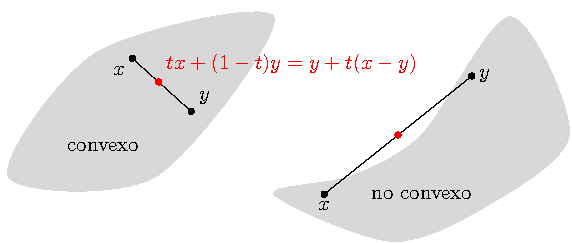
\includegraphics[width= 0.7\linewidth, page = 1]{IMAGENES/1_DEF/0/tikz.pdf}
		\end{overprint}
	\end{figure}
	\end{exampleblock}
	El resto de definiciones se darán sobre la marcha.
\end{frame}
% )))

% REPASO DE DEFINICIÓN DE ORIGAMI
\section{Origamis y Teselaciones.} % (((
\frame{\sectionpage}
\begin{frame}[t]
	\frametitle{Origami.}
	\begin{exampleblock}{}
		El \textit{\color{blue}origami} (\textit{``ori''} significa doblar, y \textit{``kami''}, significa papel), es el arte de crear superficies de papel a través de realizar \textit{dobleces} a una sola hoja. \\[2mm]
		\begin{figure}[hbtp!]
			\centering
			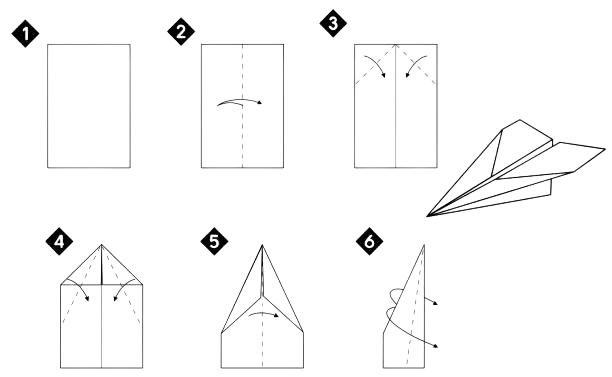
\includegraphics[width= 0.9 \linewidth]{IMAGENES/1_DEF/ex_1.png}
% TODO: Si alcanza el tiempo cambiar esta imagen por animación de tikz en la carpeta /1/
		\end{figure}
	\end{exampleblock}
\end{frame}

\begin{frame}[t]
	\frametitle{Tipos de Dobleces.}
	\begin{figure}[hbtp!]\begin{overprint}
		% \centering
		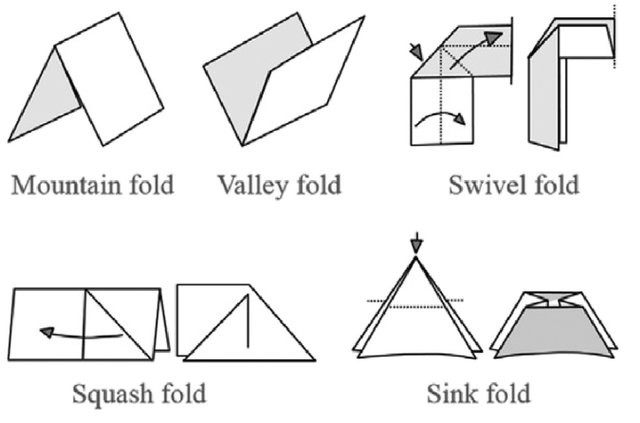
\includegraphics[width= 0.45 \linewidth, page = 1]{IMAGENES/1_DEF/tipos_1}
		\includegraphics<2>[width= 0.45 \linewidth, page = 1]{IMAGENES/1_DEF/tipos_2}
	\end{overprint}
\end{figure}
% \only<3>
	Nosotros nos concentraremos en origamis \textit{rígidos}, \textit{i.e.} sólo en aquellos donde es posible hacer dobleces \color{red} Mountain, \color{blue} Valley, \color{black} Squash y Pleat.
\end{frame}

\begin{frame}[t]
	\frametitle{Notación.}
	\begin{block}{}
		\begin{overprint}
			
\includegraphics[width=  \linewidth, page = 1]{IMAGENES/1_DEF/10/S1}
		\end{overprint}
	\end{block}
	\vspace{3mm}
\end{frame}

\begin{frame}[t]
	\begin{exampleblock}{Objetivo.}
		Esperamos convertir la superficie de papel en una superficie doblada (sin curvar las caras).
	\end{exampleblock}
	\vspace{2mm}
	\begin{exampleblock}{}
		\begin{overprint}
		\includegraphics<1>[width= \linewidth]{IMAGENES/1_DEF/2/tikz.pdf}
		% TODO: Al poner pausas habilitar ésta imagen en la misma diapositiva con <2->
		% \includegraphics<2>[width= \linewidth]{IMAGENES/1_DEF/3/tikz.pdf}
		\end{overprint}
	\end{exampleblock}
	\vspace{2mm}
	\begin{exampleblock}{}
		% \only<2>
		{Para definir un doblez, primero hagamos el doblez y veamos su marca.}
		% \only<3>
		{Entonces podemos ver a \(R = [a,b] \times [c,d]\), en \(\mathbb{R} ^3\), con \(R \times \{0\}\).}
	\end{exampleblock}
\end{frame}

\begin{frame}[t]
	\begin{block}{Definición.}
		Un \textbf{doblez en origami} es una transformación \textit{continua} \(T: [a,b] \times [c,d] \times \{0\} \longrightarrow \mathbb{R} ^3\), y esperamos que satisfaga lo siguiente.
	\end{block}
	\vspace{2mm}
	\begin{exampleblock}{}
		\begin{figure}[hbtp!]\begin{overprint}
			\centering
		\includegraphics<1>[width= \linewidth]{IMAGENES/1_DEF/3/tikz.pdf}
		% \includegraphics<2>[width= \linewidth]{IMAGENES/1_DEF/4/tikz.pdf}
		\end{overprint}
	\end{figure}
	\end{exampleblock}
	\vspace{2mm}
	\begin{exampleblock}{}
		\begin{enumerate}
			\item Existe una \textit{partición} (de polígonos convexos) \(\mathscr{A}\) de \([a,b] \times [c,d] \times \{0\}\) tal que \(T \big| _{A}\) es inyectiva para cada \(A\) en la partición \(\mathscr{A}\).
				\label{enu:1}
		\end{enumerate}
	\end{exampleblock}
\end{frame}

\begin{frame}[t]
	\begin{exampleblock}{}
		\begin{enumerate}
				\setcounter{enumi}{1}
			\item \(T \big| _A\) preserva \textit{ángulos} y \textit{distancias} entre pares de elementos de \(A\).
				\label{enu:2}
		\end{enumerate}
	\end{exampleblock}
	\vspace{2mm}
	\begin{exampleblock}{}
				% \begin{figure}[hbtp!]
					\begin{overprint}
					 \centering
					\includegraphics<1>[width= \linewidth, page = 1]{IMAGENES/1_DEF/4/tikz.pdf}
					% \includegraphics<2>[width= \linewidth, page = 1]{IMAGENES/1_DEF/5/tikz.pdf}
					% \includegraphics<3>[width= \linewidth, page = 1]{IMAGENES/1_DEF/6/tikz.pdf}
					% \includegraphics<4>[width= \linewidth, page = 1]{IMAGENES/1_DEF/7/tikz.pdf}
					\end{overprint}
				% \end{figure}
	\end{exampleblock}
	\vspace{2mm}
	\begin{exampleblock}{}
		Se tiene:
		\begin{itemize}
			\item \(arccos \bigg(\dfrac{\langle Tx-Tz,Ty-Tz\rangle}{|Tx-Tz| \cdot |Ty-Tz|}\bigg) = arccos \bigg(\dfrac{\langle x-z,y-z \rangle}{|x-z| \cdot |y-z|}\bigg)\), \(\forall x,y,z \in A\).
			\item \(\big| T  x - T   y \big| = |x-y| \;,\; \forall x,y \in A \). (\textit{i.e.} \(T \big| _A\) es una \textit{isometría}).
		\end{itemize}
	\end{exampleblock}
\end{frame}

% \begin{frame}[t]
	% \begin{exampleblock}{}
		% \begin{enumerate}
				% \setcounter{enumi}{2}
			% \item \(T \big| _A\) es \textit{lineal}, para cada \(A\) en la partición.
				% \label{enu:3}
		% \end{enumerate}
	% \end{exampleblock}
		% \vspace{2mm}
				% \begin{exampleblock}{}
				% \begin{overprint}
				% \includegraphics<1>[width= \linewidth, page = 1]{IMAGENES/1_DEF/4/tikz.pdf}
				% % \includegraphics<2>[width= \linewidth, page = 1]{IMAGENES/1_DEF/8/tikz.pdf}
			% \end{overprint}
				% \end{exampleblock}
				% \vspace{2mm}
				% \begin{exampleblock}{}
			% Esto es:
			% \begin{itemize}
				% \item \(T(ax + by) = aTx + bTy\), \(\forall x,y \in A\), y \(a,b \in \mathbb{R}\).
			% \end{itemize}
			% De tal manera que \(ax+by \in A\).
				% \end{exampleblock}
% \end{frame}

% \begin{frame}[t]
	% \begin{exampleblock}{}
		% \begin{enumerate}
			% \setcounter{enumi}{2}
		% \item Si \(T\) además manda los vértices de \(A\), a los vértices de \(T(A)\), \(\forall A \in \mathscr{A}\), entonces \(T(A)\) es convexo.
			% \label{enu:3}
		% \end{enumerate}
	% \end{exampleblock}
	% \vspace{2mm}
	% \begin{exampleblock}{}
		% Sean \(x,y \in A\), y \(z = y + t(x-y) \in A\). \\[2mm]
		% Como \(arccos \bigg(\dfrac{\langle Tx-Tz,Ty-Tz\rangle}{|Tx-Tz| \cdot |Ty-Tz|}\bigg) = arccos \bigg(\dfrac{\langle x-z,y-z \rangle}{|x-z| \cdot |y-z|}\bigg)\), \(\forall x,y,z \in A\).
		% Entonces
		% \[
			% arccos \dfrac{\langle Tx-Tz,Ty-Tz \rangle}{|Tx| \cdot |Tz|} = arccos \dfrac{t(1-t) \langle x-y,x-y \rangle}{t(1-t) |x-y| \cdot |x-y|} = 0.
		% \]
	% \end{exampleblock}
	% \vspace{2mm}
% \end{frame}

\begin{frame}[t]
	\begin{exampleblock}{}
		\begin{enumerate}
				\setcounter{enumi}{2}
			\item Si \(T \big| _A\) manda de los vértices de \(A\), a los vértices de \(T(A)\), \(\forall A \in \mathscr{A}\).
				entonces, \(area(A) = area(T(A))\).
				\label{enu:3}
		\end{enumerate}
	\end{exampleblock}
		\vspace{2mm}
			% \begin{figure}[hbtp!]
				\begin{exampleblock}{}
				\begin{overprint}
				% \centering
				\includegraphics<1>[width= \linewidth, page = 1]{IMAGENES/1_DEF/4/tikz.pdf}
				% \includegraphics<3>[width= \linewidth, page = 1]{IMAGENES/1_DEF/8.5/tikz.pdf}
				% \includegraphics<3>[width= \linewidth, page = 1]{IMAGENES/1_DEF/9/tikz.pdf}
			\end{overprint}
	% \end{figure}
					(Notamos que no podemos usar la medida de Lebesgue para obtener el área, ni \(detT \big| _A\) en caso de que \(T \big| _A\) fuera lineal).\\
					Si \(A \in \mathscr{A}\), consideremos una división de \(A\) por triángulos.
					Usamos la \textit{fórmula de Herón}: Si \(D\) es un triángulo de lados \(a,b,c\), y \(s=(a+b+c)/2\), entonces \(area(D) = \sqrt{s(s-a) (s-b) (s-c)}\).
				\end{exampleblock}
\end{frame}

\begin{frame}[t]
	\begin{exampleblock}{}
		Sean entonces \(\mathscr{D} = \{D_i \;|\; i \leqslant n_A\}\) una partición de \(A\), por triángulos.\\
		Probemos que \(T(\mathscr{D}) = \{T(D_i) \;|\; i \leqslant n_A\}\) es una partición de \(T(A)\).
		\begin{itemize}
			\item \(A = \dis\bigcup_{i=1}^{n_A} D_i\).
			\item \(\forall i \ne j \;\implies\; D_i \cap D_j = \varnothing\).
		\end{itemize}
		Luego,
		\begin{itemize}
			\item \(T(A) = T \Bigg(\dis\bigcup_{i=1}^{n_A} D_i\Bigg) = \dis\bigcup_{i=1}^{n_A} T(D_i)\).
			\item Como \(T\) es inyectiva en \(A\),
				\[
					T(D_i) \cap T(D_j) = T(D_i \cap D_j) = T(\varnothing) = \varnothing .
				\]
		\end{itemize}
		Así \(T(\mathscr{D})\) es partición de \(T(A)\).
		Sean \(x,y,z\) los vértices de \(D_i\). Sea \(a = |x-y| , b =|y-z|, c = |x-z|\), entonces con \(s = (a+b+c) /2\),
		\[
			area(D_i) = \sqrt{s(s-a) (s-b) (s-c)}.
		\]
	\end{exampleblock}
\end{frame}

\begin{frame}[t]
	\begin{exampleblock}{}
		Como \(T(\{x,y,z\})\) son los vértices de \(T(D_i)\), y es isometría
		\(\left| Tx - Ty \right| = |x-y| = a\),\\
		\(\left| Ty - Tz \right| = |y-z| = b\),\\
		\(\left| Tx - Tz \right| = |x-z| = c\).
		Por la fórmula de Herón,
		\[
			area(D_i) = area(T(D_i)) \;,\;  \forall i \leqslant n_A.
		\]
		Y como \(\mathscr{D}\) es partición de \(A\).
		\[
			area(A) := \dis\suma_{i=1}^{n_A} area(D_i).
		\]
		Al ser \(T(\mathscr{D})\) partición de \(T(A)\),
		\[
			area(T(A)) := \dis\suma_{i=1}^{n_A} area(T(D_i)) = \dis\suma_{i=1}^{n_A} area(D_i) = area(A). \qed
		\]
	\end{exampleblock}
\end{frame}

\begin{frame}[t]
	\begin{exampleblock}{}
		Más aún, cada doblez debe tener una relación de homotopía.
	\end{exampleblock}
	\vspace{2mm}
	\begin{exampleblock}{}
		\begin{overprint}
			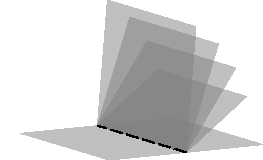
\includegraphics[width= 0.6\linewidth, page = 1]{IMAGENES/1_DEF/11/tikz.pdf}
		\end{overprint}
	\end{exampleblock}
	\vspace{2mm}
	\begin{exampleblock}{}
		Es decir, debe existir \(H: A \times [0,1] \longrightarrow \mathbb{R} ^3\) continua, tal que
		\begin{enumerate}
			\setcounter{enumi}{3}
		\item \(\forall t \in [0,1]\), \(T_t: A \longrightarrow \mathbb{R} ^3\), por \(T_t(x) = H(x,t)\), es una función continua que satisface las propiedades  \Myref{enu:1}, \Myref{enu:2} y \Myref{enu:3}.
		\end{enumerate}
	\end{exampleblock}
	Observar que no estamos dando las reglas de correspondencia de \(T\) y \(H\) explícitamente. Sólo son las propiedades que se requieren satisfacer.
\end{frame}

\begin{frame}[t]
	\begin{block}{Observación.}
		Las definiciones anteriores fueron dadas para un sólo doblez.
		Sin embargo, se cumplen para todo el conjunto de funciones que aplican un doblez nuevo sobre \([a,b] \times [c,d] \times \{0\}\),
		o sobre \(T([a,b] \times [c,d] \times \{0\})\).
		\begin{enumerate}
			\item La composición de isometrías es isometría.
				\[
					\big| TUx - TUy \big| = \big| Ux - Uy \big| = |x-y|.
				\]
			\item La composición de funciones que preservan ángulos, preserva ángulos.
				\[
					arccos \dfrac{\langle TUx,TUy \rangle}{|TUx| \cdot |TUy|} = arccos \dfrac{\langle Ux,Uy \rangle}{|Ux| \cdot |Uy|} = arccos \dfrac{\langle x,y \rangle}{|x| \cdot |y|}.
				\]
			\item La composición de dos funciones que mandan vértices a vértices, manda de vértices a vértices.
			\item Si \(U,T\) son inyectivas, mandan una partición \(\mathscr{A}\) a una partición en \(T(\mathscr{A})\). Su composición es inyectiva.
		\end{enumerate}
	\end{block}
	\vspace{2mm}
\end{frame}

\begin{frame}[t]
	\begin{exampleblock}{}
		\begin{enumerate}
				\setcounter{enumi}{4}
			\item Si \(A\) y \(T(A)\) satisfacen una relación de homotopía, y \(T(A)\) y \(UT(A)\) satisfacen una relación de homotopía, entonces \(A\) y \(UT(A)\) también.
				Considérese \(H(x,t) = H_T(x,2t),\) para \(t \in [0,1/2]\), \(H(x,t) = H_U(x,2t-1)\), para \(t \in [1/2,1]\). \\[2mm]
				Siempre y cuando \(H_T(x,1) = H_U(x,0)\), \(\forall x \in [a,b] \times [c,d] \times \{0\}\).
		\end{enumerate}
	\end{exampleblock}
	\vspace{2mm}
\end{frame}

\begin{frame}[t]
	\frametitle{Teselaciones.}
	\begin{block}{Definición.}
		Una teselación es una partición de \(\mathbb{R} ^2\), con figuras repetidas.
	\end{block}
	\vspace{2mm}
	\begin{exampleblock}{}
		\begin{overprint}
			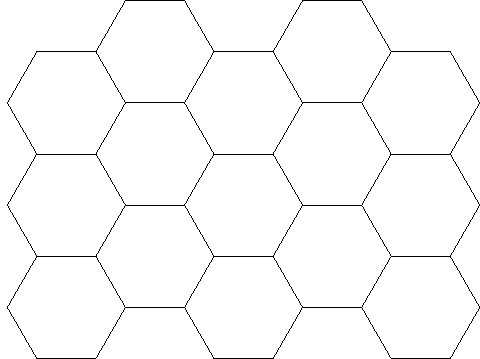
\includegraphics[width= 0.7\linewidth, page = 1]{IMAGENES/1_DEF/12/tikz.pdf}
		\end{overprint}
	\end{exampleblock}
\end{frame}

\begin{frame}[t]
	\begin{block}{Teorema.}
		Sólo hay tres polígonos regulares capaces de particionar el plano.
		\begin{enumerate}
			\item Los triángulos equiláteros.
			\item Los cuadrados.
			\item Los hexágonos.
		\end{enumerate}
	\end{block}
	\vspace{2mm}
	\begin{block}{Demostración.}
		\begin{minipage}{0.6\linewidth}
		Sea \(P_n\) el polígono regular con \(n\) lados.\\
		Sea \(\alpha (n)\) su ángulo interior.\\
		Debe existir \(k \in \mathbb{N}\), tal que \(k \alpha (n) = 2 \pi\).\\
			La suma de ángulos exteriores es \(2 \pi\), \textit{i.e.} \\[-3mm]
			\[
				\dis\suma_{i=1}^{n} (\pi - \alpha (n)) = 2 \pi .
			\]
			Entonces \(n(\pi - \alpha (n)) = 2 \pi\).\\
			\(\alpha (n) = \pi - \dfrac{2 \pi}{n} = (2 \pi) \dfrac{n - 2}{2n}\).
		\end{minipage}
		\begin{minipage}{0.3\linewidth}
			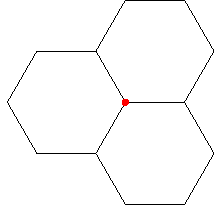
\includegraphics[width= \linewidth, page = 1]{IMAGENES/1_DEF/13/tikz.pdf}
		\end{minipage}
	\end{block}
\end{frame}

\begin{frame}[t]
	\begin{exampleblock}{}
		Entonces \(2 \pi / \alpha (n) = \dfrac{2n}{n-2} = k \in \mathbb{N}\).
		Grafiquemos a sucesión.
	\end{exampleblock}
	\vspace{2mm}
	\begin{exampleblock}{}
		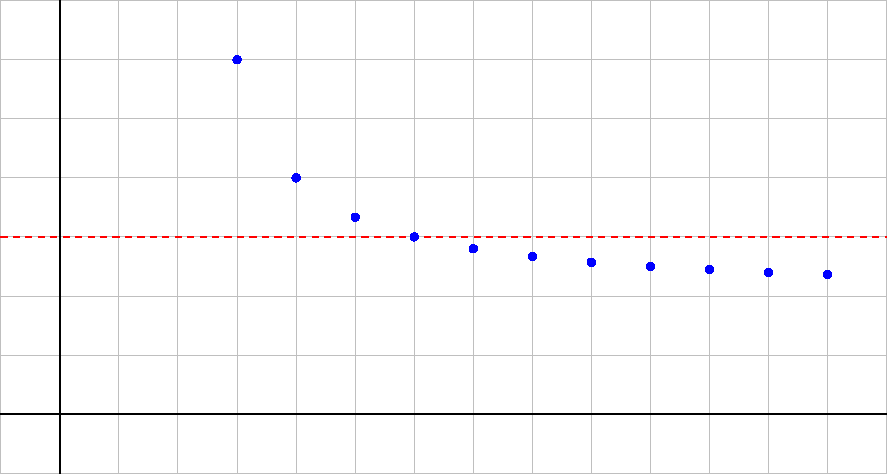
\includegraphics[width= 0.9 \linewidth, page = 1]{IMAGENES/1_DEF/14/tikz.pdf}
	\end{exampleblock}
	\vspace{2mm}
	\begin{exampleblock}{}
		Notamos que \(n = 3,4,6\), son los únicos valores para \(k \in \mathbb{N}\).
		Dado que \(\forall n>6\), \(k = \dfrac{2n}{n-2} \in (2,3)\), y \(\dis\lim_{n\rightarrow \infty} \dfrac{2n}{n-2} = 2\).
	\end{exampleblock}
	\vspace{2mm}
\end{frame}
% )))

% INTRODUCCIÓN A MANIFOLDS (con animaciones)
\section{Problema a Resolver.} % (((
\frame{\sectionpage}
\begin{frame}[t]
	\frametitle{Manifold. The Origami Mindbender.}
	\begin{exampleblock}{}
		El juego de origami de Brainwright\texttrademark, Manifold\textcopyright, es un producto de 100 rejillas de papel $8\times 8$ coloreadas de forma diferente por un único lado. 
		\begin{figure}[hbtp!]\begin{overprint}
			\centering
			\includegraphics<1>[width= 0.8 \linewidth, page = 1]{IMAGENES/2_PROB/1/producto_3.png}
		\end{overprint}
	\end{figure}
	El objetivo es que por medio de dobleces se consiga construir una rejilla $4\times 4$, con una cara blanca, y que su reverso conste de una cara negra.
	\end{exampleblock}
	\vspace{2mm}
\end{frame}

\begin{frame}[t]
	\frametitle{Ejemplos.}
	\begin{figure}[hbtp!]\begin{overprint}
		\centering
		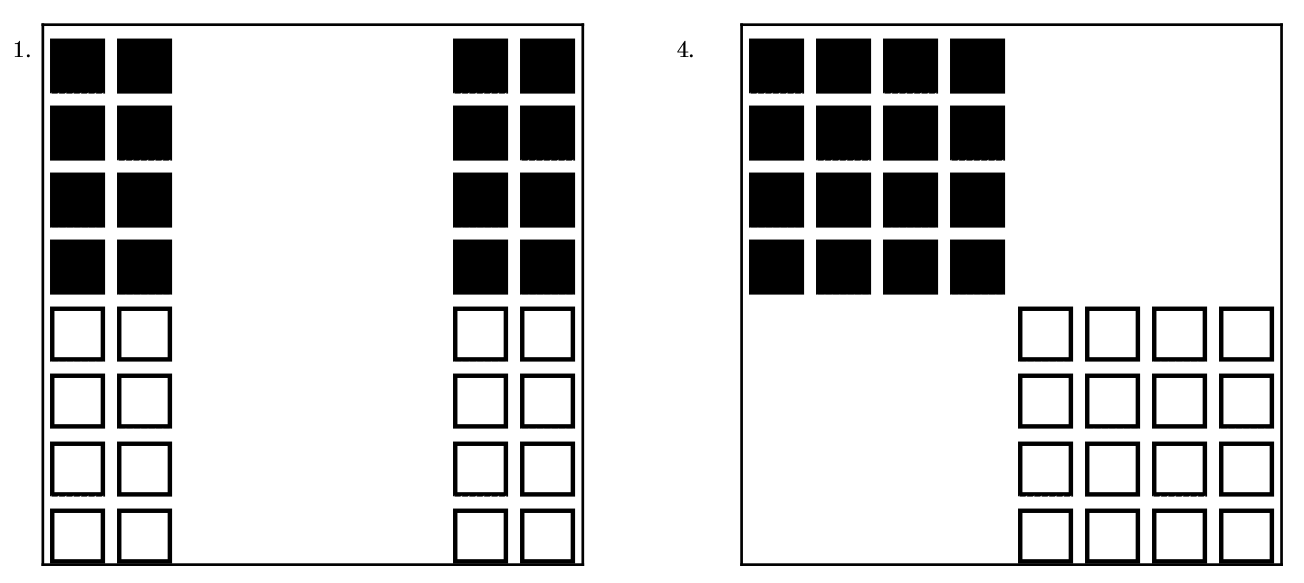
\includegraphics[width= \linewidth, page = 1]{IMAGENES/2_PROB/2/1}
	\end{overprint}
\end{figure}
\end{frame}

\begin{frame}[t]
	\frametitle{Ejemplos.}
	\begin{figure}[hbtp!]\begin{overprint}
		\centering
		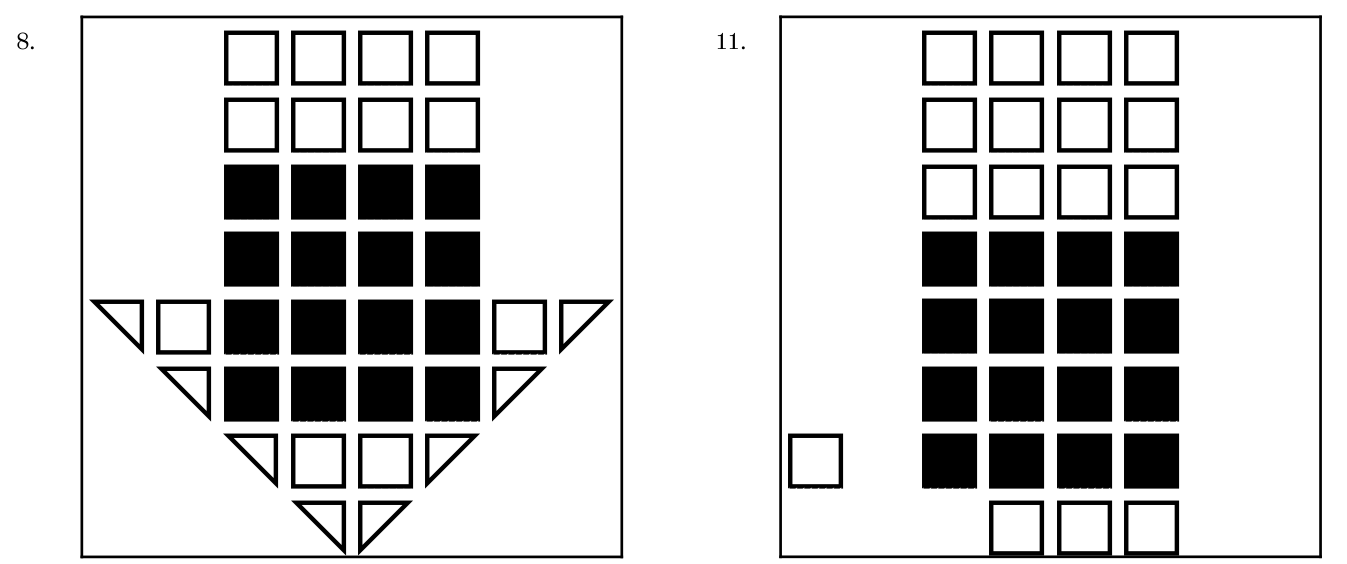
\includegraphics[width= \linewidth, page = 1]{IMAGENES/2_PROB/2/2}
	\end{overprint}
\end{figure}
\end{frame}

\begin{frame}[t]
	\frametitle{Ejemplos.}
	\begin{figure}[hbtp!]\begin{overprint}
		\centering
		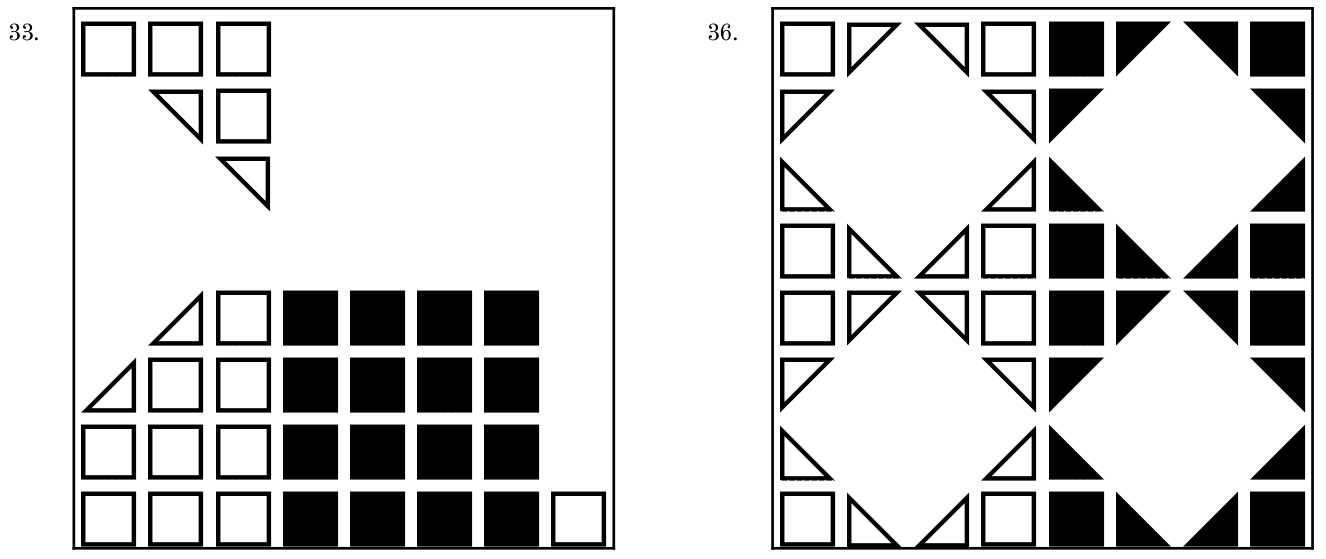
\includegraphics[width= \linewidth, page = 1]{IMAGENES/2_PROB/2/3}
	\end{overprint}
\end{figure}
\end{frame}

\begin{frame}[t]
	\frametitle{Ejemplos.}
	\begin{figure}[hbtp!]\begin{overprint}
		\centering
		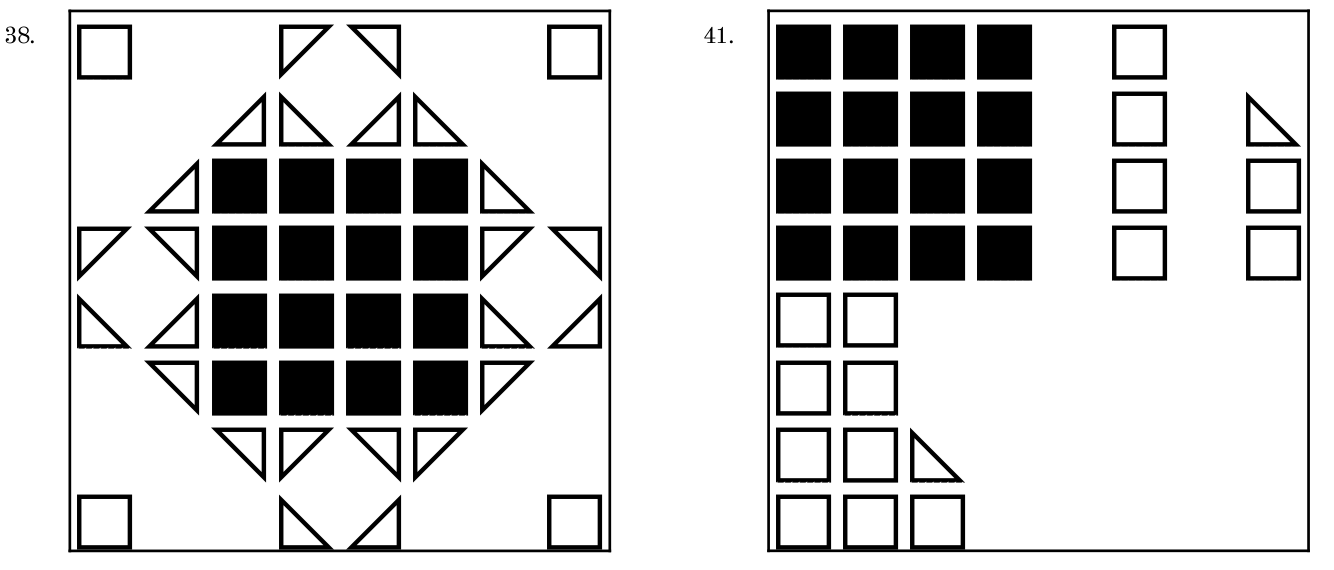
\includegraphics[width= \linewidth, page = 1]{IMAGENES/2_PROB/2/4}
	\end{overprint}
\end{figure}
\end{frame}

\begin{frame}[t]
	\frametitle{Ejemplos.}
	\begin{figure}[hbtp!]\begin{overprint}
		\centering
		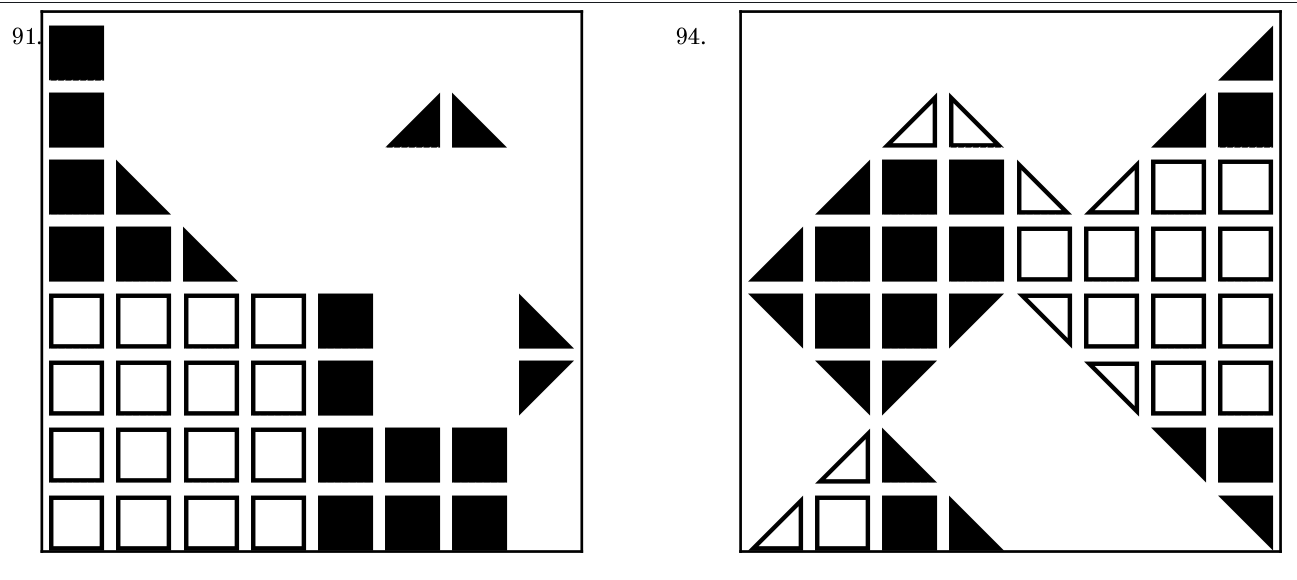
\includegraphics[width= \linewidth, page = 1]{IMAGENES/2_PROB/2/5}
	\end{overprint}
\end{figure}
\end{frame}

\begin{frame}[t]
	\frametitle{Ejemplos.}
	\begin{figure}[hbtp!]\begin{overprint}
		\centering
		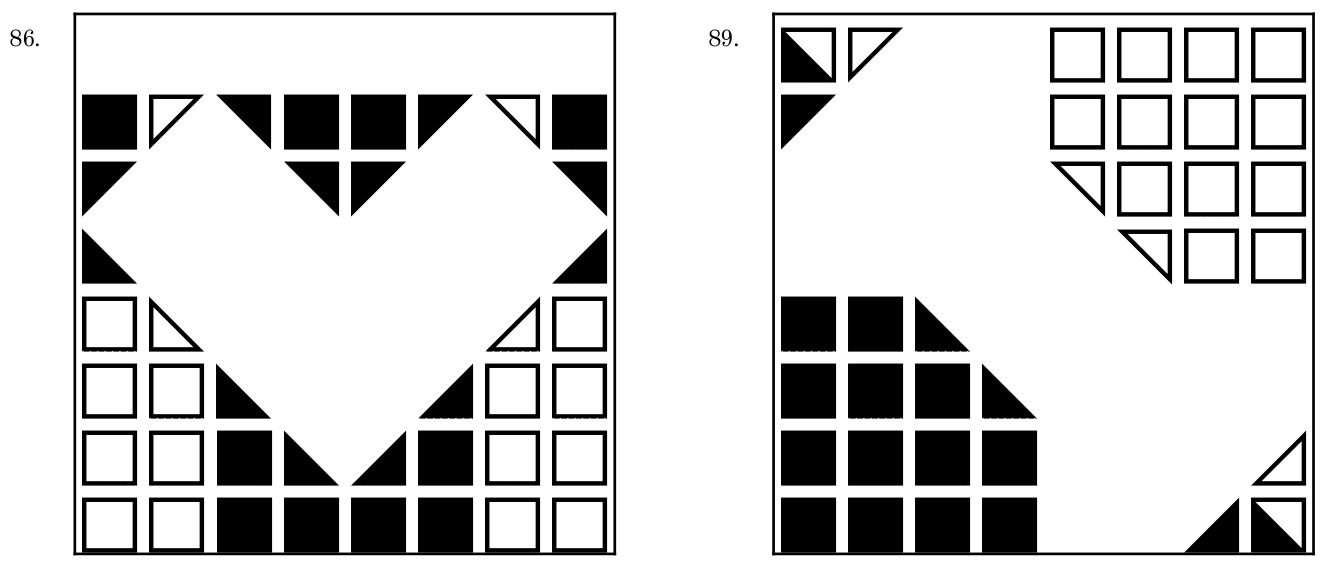
\includegraphics[width= \linewidth, page = 1]{IMAGENES/2_PROB/2/6}
	\end{overprint}
\end{figure}
\end{frame}

% )))

\section{Primeros intentos.} % (((
\frame{\sectionpage}
% Primer intento de definir doblez (con JM, en triangulos).
\begin{frame}[t]
	\frametitle{Primer Intento.}
	\begin{block}{Definición.}
		Sea \(V \ne \varnothing\). Un \textbf{grafo} es un par \((V,E)\), donde \(E \subseteq V^2\).
	\end{block}
	\vspace{3mm}
	\begin{example}
		Sea \(V = \{1, \;\ldots,\; 7\}\), y \(E = \big\{\; \{1,2\} \;,\; \{1,5\} \;,\; \{2.5\} \;,\; \{3,4\} \;,\; \{5,7\}\big\}\), se representa de la siguiente forma.
		\begin{figure}[hbtp!]
			\centering
			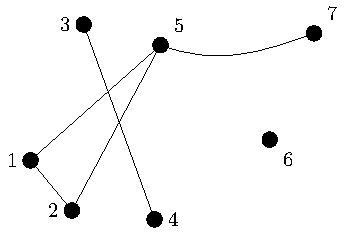
\includegraphics[width= 0.5 \linewidth, page = 1]{IMAGENES/3_INT/1/tikz.pdf}
		\end{figure}
	\end{example}
\end{frame}

\begin{frame}[t]
	\begin{block}{Primer Intento.}
		Consideremos los siguientes subconjuntos en \(\mathbb{R} ^2\).
		\begin{figure}[hbtp!]
			\centering
			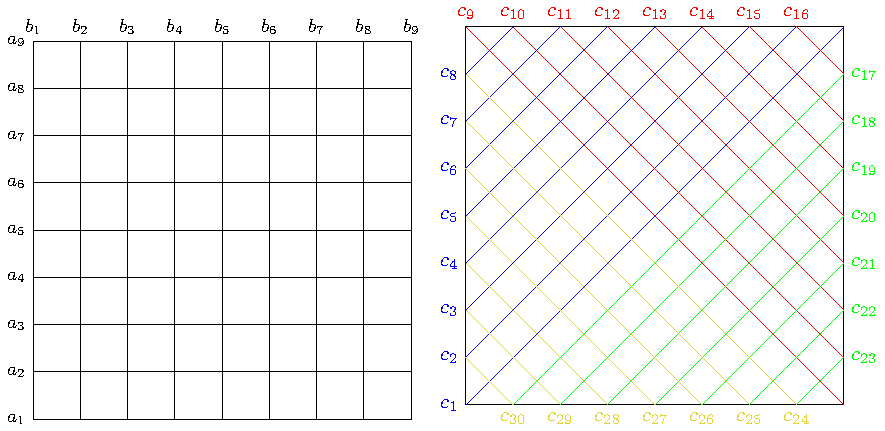
\includegraphics[width= 0.9 \linewidth, page = 1]{IMAGENES/3_INT/2/tikz.pdf}
		\end{figure}
	\end{block}
\end{frame}

% teselaciones cuadradas.
\begin{frame}[t]
	\frametitle{Reducción del Problema.}
\end{frame}

% Segundo intento (con alfileres)
\begin{frame}[t]
	\frametitle{Segundo Intento.}
\end{frame}

% tercer intento (funciones indicadoras) + Teorema
\begin{frame}[t]
	\frametitle{Tercer Intento.}
\end{frame}

% papers (map foldings) (+ 1 teorema desmotrado)
\begin{frame}[t]
	\frametitle{Map Foldings.}
\end{frame}

% intento de definir topología (spoiler resulta la discreta)-
\begin{frame}[t]
	\frametitle{Cuarto Intento.}
\end{frame}

% Grafos (matriz de adyacencia).
\begin{frame}[t]
	\frametitle{Matriz de Adyacencia.}
\end{frame}
% )))

% pi-sistemas
\section{Pi-Sistemas.} % (((
\frame{\sectionpage}
\begin{frame}[t]
	\frametitle{Pi-Sistemas.}
	\begin{block}{Observación.}
		\begin{minipage}{0.5\linewidth}
			La intersección de rectángulos siempre es un rectángulo. \\[2mm]
			La unión de rectángulos no-necesariamente es rectángulo.
			\[
				\bigg(\dis\bigcup_{i=1}^{n} A_i\bigg) \times \bigg(\dis\bigcup_{i=1}^{m} B_i\bigg) = \dis\bigcup_{i,j = 1}^{n,m} A_i \times B_j.
			\]
			Es decir, no se puede definir una topología cuyos abiertos sólo sean rectángulos.
		\end{minipage}\hspace{5mm}
		\begin{minipage}{0.4\linewidth}
			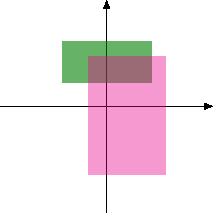
\includegraphics[width= \linewidth, page = 1]{IMAGENES/4_PI/1/tikz.pdf}
		\end{minipage}
	\end{block}
\end{frame}

\begin{frame}[t]
	\begin{block}{Definición.}
		Sea \(X \ne \varnothing\). Una colección \(\mathscr{C} \subseteq \mathscr{P}(X)\), es un \textbf{\(\pi\)--sistema} si satisface la siguiente condición.
		\begin{enumerate}
			\item \(\forall A_1, \;\ldots,\; A_n \in \mathscr{C} \;\implies\; \dis\bigcap_{i=1}^{n} A_i \in \mathscr{C}\).
		\end{enumerate}
	\end{block}
	\vspace{3mm}
	\begin{block}{Lema.}
		Sea \(\mathscr{A}\) conjunto de índices. Si \(\mathscr{C} _\alpha\), \(\alpha \in \mathscr{A}\) es un \(\pi \)--sistema, para todo \(\alpha \in \mathscr{A}\), entonces \(\dis\bigcap_{\alpha \in \mathscr{A}} \mathscr{C}_\alpha \mbox{ es un } \pi \mbox{--sistema.}\) \\[2mm]
		\textbf{Demostración.}
		\begin{itemize}
			\item Si \(A_1, \;\ldots,\; A_n \in \dis\bigcap_{\alpha \in \mathscr{A}} \mathscr{C} _\alpha\), entonces
			\item \(A_1, \;\ldots,\; A_n \in \mathscr{C} _\alpha\), \(\forall \alpha \in \mathscr{A}\). Por ser \(\mathscr{C} _\alpha\), \(\pi\)--sistema:
			\item \(\dis\bigcap_{i=1}^{n} A_i \in \mathscr{C} _\alpha\), \(\forall \alpha \in \mathscr{A}\). Por tanto \(\dis\bigcap_{i=1}^{n} A_i \in \dis\bigcap_{\alpha \in \mathscr{A}} \mathscr{C} _\alpha\). \qed
		\end{itemize}
	\end{block}
\end{frame}
% PI SISTEMAS QUE SE PUEDEN DEFINIR:
% BARRAS HORIZONTALES - BARRAS VERTICALES - SIGNLETONS
% RECTÁNGULOS 2 X 2 - SINGLETONS
% RECTANGULOS N x M EN GENERAL.
% )))

% definir con una operación (algebra).
\section{Álgebra.} % (((
\frame{\sectionpage}
\begin{frame}[t]
	\frametitle{El Grupo Simétrico.}
	\begin{block}{Definición.}
		Sea \(G \ne \varnothing\). Un \textbf{grupo} es un par \((G,f)\) donde \(f:G^2 \longrightarrow G\), con las siguientes propiedades.
		\begin{enumerate}
			\item \(f(f(a,b) ,c) = f(a,f(b,c))\), \(\forall a,b,c \in G\).
			\item \(\exists e \in G \;:\; f(a,e) = f(e,a) = a\), \(\forall a \ne G\).
			\item \(\forall a \in G \;,\; \exists b \in G \;:\; f(a,b) = f(b,a) = e\).
		\end{enumerate}
	\end{block}
\end{frame}
% )))

% TODO:
% === REFERENCIAS === (((
% )))

% TODO: si sobra tiempo ver con variable compleja.

\end{document}
